%ब
\section{Referential Integrity in Key-Value
Model}\label{s:referential-integrity} 

Referential integrity is a fundamental property of data within databases, which
ensures that data dependencies between tables are maintained correctly in the
database~\citep{blaha,date,Navathe,george}.  These dependencies are generally a
part of the business rule and are enforced using referential integrity
constraints to ensure proper data integrity. These  constraints
have been a relational feature in traditional \acp{RDBMS} and are imposed due to
the way the \acp{RDBMS} enforce normalisation. Such  constraints are defined on
the tables in a database, and have to be mandatorily satisfied at all times in
order to ensure that users or applications do not enter incorrect or
inconsistent data into the databases.



Generally in \acp{RDBMS}, referential integrity constraints  ensure that the
value of foreign keys in a table matches the values of primary keys in another
table. That is, referential integrity is enforced by the combination of a
primary (or unique) key and a foreign key such that every foreign key matches
the primary key~\citep{blaha,Navathe,george,pathivada}.
In the University example,   every foreign key in the \texttt{Enrolment} table
must match one of the primary keys in the \texttt{Student} and \texttt{Course}
tables. Hence,   if any foreign key refers to a non-existing primary key,   the
referential integrity constraint is violated.   For example,   if
'\texttt{StudID100}' is a foreign key for a student in the \texttt{Enrolment}
table,   but '\texttt{StudID100}' does not exist as a primary key in the
\texttt{Student} table,   it is a violation of referential integrity.
Notice that the table containing the foreign key is the referencing table (or
child table), while the table with the primary or unique key is the referenced
table (or parent table). For example,  \texttt{Enrolment} is the referencing
table while \texttt{Student} and \texttt{Course} are the referenced tables.
Foreign keys are also known as  referencing keys and the primary keys as
referenced keys.



% In order to improve the data dependency in cloud \ac{NoSQL} \acp{DBMS},   this
% thesis proposes solutions that implement referential integrity constraints using
% different approaches. These solutions are deployed and evaluated using Apache
% Cassandra, a column-oriented key-value cloud Database Management System (DBMS).
% The following section gives an overview of Cassandra and discusses some of its
% key architectural concepts.

 
Referential integrity constraints also describe the data manipulation that is
allowed on the referenced values.  Some of the widely associated rules are:

	\begin{itemize}	
		\item \texttt{Restrict} or \texttt{No delete}: which prevents any update or
		deletion of data that has references. 		
		\item \texttt{Set to NULL}: which sets all foreign keys to NULL values,   on
		updating or deleting the referenced key. 		
		\item \texttt{Set to Default}: which sets all the foreign
		keys to a default value,   on updating or deleting the referenced key. 		
		\item \texttt{Cascade}: which updates or deletes all the
		associated dependant values accordingly,   when the referenced data is updated or
		deleted. 		
		\item \texttt{No Action}: which performs checks only at the end of a
		statement and is similar to \texttt{Restrict}		
	\end{itemize}

Existing \acp{DBMS} may not always support all of the above rules.  Some \acp{DBMS} may
have the \texttt{Cascade} rule by default like Oracle,   while some may have the
\texttt{Restrict} rule by default.  

Generally,   in \acp{RDBMS} the database manager enforces a set of rules to
prevent any data operation,   like insert,   update or delete,   to change data
in such a way that referential integrity is not violated as seen in
Figure~\ref{f:RI}. 

	\begin{figure}[H]
		\centering
		%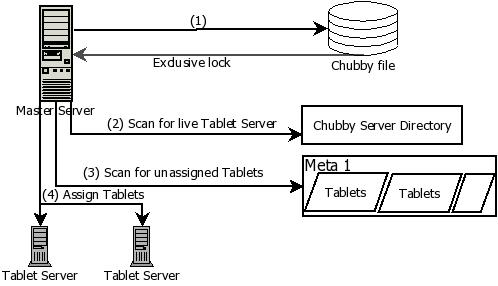
\includegraphics[width=5cm,   height=5cm]{. /figure/random. jpg}
		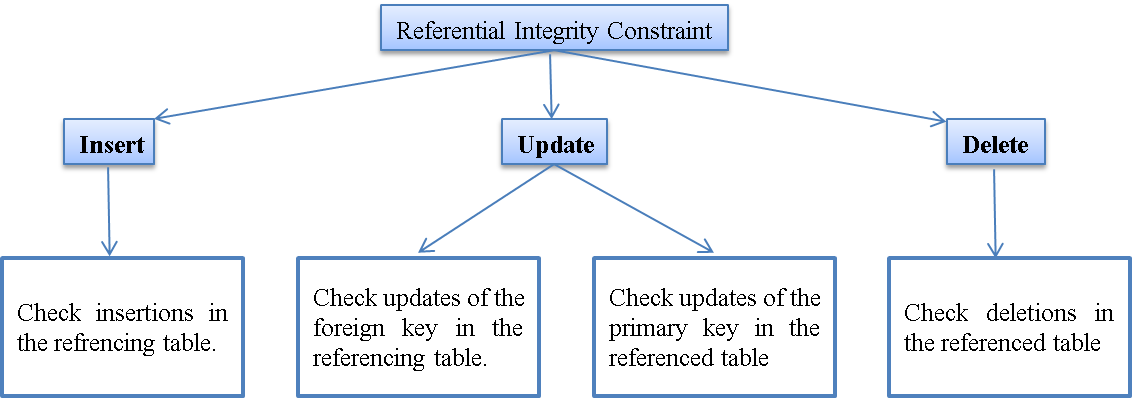
\includegraphics[width=.8\textwidth]{./figure/Example/RI-Figure.png}
		\caption{Referential Integrity Rules}\label{f:RI}
	\end{figure}



% These rules are explained below:

% 	\begin{itemize}
\subsection{Insert rule}
		An insert operation triggers a referential integrity
		validation when data is being inserted into a referencing table,   i. e. ,   the
		child table.  In such an event,   prior to entering the values in the
		referencing table,   it is checked if the foreign keys exist in the referenced
		table.  For example,   in the University \ac{RDB},   when a row is inserted in
		the \texttt{Enrolment} table with foreign key values for \texttt{StudentID} and
		\texttt{CourseID},   a check is triggered to verify whether these foreign keys
		exist in the \texttt{Student} and \texttt{Course} tables as primary keys.  If
		the foreign keys do not exist in the referenced tables,   then the insert
		operation is not allowed.
		
\subsection{Update rule}
 When data is updated either in the referencing table or the
		referenced table,   a referential integrity validation is required.  When any
		primary key is updated in the referenced table, then it is verified whether this
		key is a foreign key in any of the referencing tables.  If a dependency is found
		to exist in the referencing tables,   then the applicable data manipulation
		rule is checked.
		For instance,   if it is a \texttt{Cascade} rule,   then the associated foreign keys
		in the referencing table are updated prior to updating the primary key in the
		referenced table.  Consider the University \ac{RDB}, if the primary key
		'\texttt{SWEN100}' for a course is updated to '\texttt{SWEN101}',   then all the records in
		\texttt{Enrolment} that have '\texttt{SWEN100}' as a foreign key are
		updated to '\texttt{SWEN101}', if it has a \texttt{Cascade} rule.
		
		When any foreign key is  updated in a referencing table,   then a
		referential integrity validation has to be performed.  It is ensured that the
		new updated value exists as a primary key in the referenced table.  For example,
		  in the \texttt{Enrolment} table,   if \texttt{CourseID} in a row is updated to
		a new value,   then it is verified that the new value is an existing primary key
		in the \texttt{Course} table.  If the new value does not exist,   the update is
		not allowed generally.
		
\subsection{Delete rule} A delete operation triggers a referential integrity
		validation when data is deleted from the referenced table.  When data that is
		marked for deletion is found to have dependencies in other referencing tables,  
		the data manipulation rule applicable for this operation is checked. 
		That is, if the rule is \texttt{Cascade},   then the depending values
		in the referencing table have to be removed prior to deleting values from the
		referenced tables.  For example,   when a student record is deleted from the
		\texttt{Student} table,   a check is performed to see if the
		\texttt{StudentID} is a foreign key in any other table.  Therefore,  
		\texttt{Enrolment} is checked and when the \texttt{StudentID} is found
		as a foreign key,   the appropriate action is performed depending on the data
		manipulation rule.  If it is \texttt{Cascade},   the enrolment details for the
		\texttt{StudentID} are removed from \texttt{Enrolment} and then the student
		record is deleted from 	\texttt{Student}. 
	
% 	\end{itemize}


 

